 \chapter[Structure with two neutrons]{Nuclear Structure with two--nucleon transfer}\label{C8}
 In what follows, we apply the formalism worked out in the previous chapter with the help of software developed to calculate absolulte two--particle transfer differential cross sections, associated with reactions induced by both light and heavy ions (cf. App. \ref{C8AppD} \textsc{cooper}, \textsc{one}).
 A number of examples are treated with special detail. Namely, two--particle transfer in light pairing vibrational nuclei, including the halo unstable nucleus $^{11}$Li, in superfluid medium heavy nuclei lying along the stability valley (Sn--isotopes) and in heavy closed shell  systems (Pb). In this last case both for  light and heavy ion projectiles.
 \section[Evidence for phonon mediated pairing]{The $^1$H($^{11}$Li,$^9$Li)$^3$H reaction: evidence for phonon mediated pairing}\label{C8S1}
    \begin{figure}
    \centerline{\includegraphics*[width=16cm,angle=0]{C8/figsC8/fig8_1_3x}}
    	\caption{\emph{Gedanken} (two--particle transfer) coincidence experiments aimed at better individuating the couplings involved in the neutron halo Cooper pair correlations in $^{11}$Li and of the $1/2^-$ first excited state of $^9$Li populated in the  
    	 $^1$H($^{11}$Li,$^9$Li)$^3$H  reaction (\cite{Barranco:01,Potel:10}). From \cite{Potel:14}.}\label{fig8_1_3}
    \end{figure}
 \begin{figure}
 \centerline{\includegraphics*[width=15cm,angle=0]{C8/figsC8/fig8_1_1}}
 	\caption{Schematic representation of the bare nucleon-nucleon and phonon induced pairing correlations (upper part) NFT diagrams, and of the population of the first, excited state of $^{9}$Li($1/2^{-}; 2.69$ MeV), in the TRIUMF experiment  reported in ref. \cite{Tanihata:08}.}\label{fig8_1_1}
 \end{figure}
 We start by discussing  the analysis of the two--neutron pickup reaction $^1$H($^{11}$Li,$^9$Li)$^3$H \citep{Tanihata:08}. Particular  attention is paid to the  excitation of the $1/2^-$ first excited state of $^9$Li lying at 2.69 MeV (cf. Figs. \ref{fig8_1_3} and \ref{fig8_1_1}). To assess the direct character of the $1/2^-$ excitation process, the importance of inelastic (cf. Apendice 1E de la introduccion inelastic scattering) and knockout (cf. Ch.\ref{C6}) channels were considered and found to be small (see App. \ref{C8AppB}). The results thus provide evidence for a new mechanism of pairing correlations in nuclei: pigmy resonance mediated pairing interaction (\citet{Barranco:01}, see also App. \ref{C8AppA}), which strongly renormalizes the bare, $NN$--$^1S_0$ interaction \citep{Potel:10}. This is but a particular embodiment of phonon mediated pairing interaction found throughout in nuclei (cf. e.g. \citet{Barranco:99,Gori:04} cf. also \citet{Brink:05}). The main difference between light halo exotic nuclei and medium heavy superfluid nuclei lying along the valley of stability is the role fluctuations play in dressing particles (quasiparticles) and in renormalizing their properties (mass, charge, etc.) and their interactions.
  \begin{figure}
  \centerline{\includegraphics*[width=18cm,angle=0]{C8/figsC8/fig8_1_3}}
  	\caption{Absolute, two--nucleon transfer differential cross section associated with the ground state and the first 	excited state of $^9$Li, excited  in the reaction $^1$H($^{11}$Li,$^9$Li)$^3$H \citep{Tanihata:08} in comparison with the predicted differential cross sections \citep{Potel:10} calculated making use of spectroscopic amplitudes and Cooper pair wavefunctions calculated in NFT.}\label{fig8_1_2}
  \end{figure}
 In fact, in the case of e.g. Sn isotopes, mean field effects are dominant, while in the case of halo exotic nuclei renormalization effects can be as large as mean field ones. 

 
 
 
 
 
 

\subsection{Structure}
Within the scenario presented in Chapter \ref{chapter1}  (App. \ref{App1AF}) and Chapter \ref{C6} (Sect. \ref{C6S2.2x}) the wavefunction describing the structure of the halo neutrons in the ground state of $^{11}$Li (the $p_{3/2}$ proton being assumed to act only as a spectator) can be written as
\begin{equation}\label{eq8_2_1}
|0\rangle_\nu=|0\rangle+\alpha|(p_{1/2},s_{1/2})_{1^-}\otimes 1^-;0\rangle+\beta|(s_{1/2},d_{5/2})_{2^+}\otimes 2^+;0\rangle,
\end{equation}
with
\begin{equation}\label{eq8_2_2}
\alpha=0.7,\quad \text{and} \quad \beta=0.1,
\end{equation}
and
\begin{equation}\label{eq8_2_3}
|0\rangle=0.45|s_{1/2}^2(0)\rangle+0.55|p_{1/2}^2(0)\rangle+0.04|d_{5/2}^2(0)\rangle,
\end{equation}
$|1^-\rangle$ and $|2^+\rangle$ being the (RPA) states describing the dipole pigmy resonance of $^{11}$Li and the quadrupole vibration of the core. While these states are virtual excitations which, exchanged between the two neutrons bind them to the Fermi surface provided by the $^9$Li core, they can be forced to become real with the help of the specific probe of Cooper pairs in nuclei, namely two--particle transfer reactions (Figs. \ref{fig8_1_1} and \ref{fig8_1_2}).
\begin{table}[h!]
%\caption{Optical model parameters used in the two--neutron transfer calculations}
{\begin{tabular}{|c|c|c|c|c|c|c|c|c|c|c|c|c|}
\cline{2-13} 
\multicolumn{1}{c|}{}& \multicolumn{12}{|c|}{$^{11}$Li($p,t)^{9}$Li}           \\
\cline{2-13} 
\multicolumn{1}{c|}{} & $V$ & $W$ &  $V_{so}$ &  $W_d$ &  $r_1$ &  $a_1$ &  $r_2$ &  $a_2$ &  $r_3$ &  $a_3$ &  $r_4$ &  $a_4$            \\
\hline 
$p$,\;$^{11}$Li$\,^{d)}$ & $63.62$ & $0.33$ &  $5.69$ &  $8.9$ &  $1.12$ &  $0.68$ &  $1.12$ &  $0.52$ &  $0.89$ &  $0.59$ &  $1.31$ &  $0.52$ \\
\hline 
$d$,\;$^{10}$Li$\,^{b)}$ & $90.76$ & $1.6$ &  $3.56$ &  $10.58$ &  $1.15$ &  $0.75$ &  $1.35$ &  $0.64$ &  $0.97$ &  $1.01$ &  $1.4$ &  $0.66$ \\
\hline 
$t$,\;$^{9}$Li$\,^{c)}$ & $152.47$ & $12.59$ &  $1.9$ &  $12.08$ &  $1.04$ &  $0.72$ &  $1.23$ &  $0.72$ &  $0.53$ &  $0.24$ &  $1.03$ &  $0.83$ \\
\hline 

\hline 
  \end{tabular}}
   \caption{Optical potentials (cf. \cite{Tanihata:08}) used in the calculation of the absolute differential cross sections displayed in Fig. \ref{fig8_1_2}.}
\label{tab8.1.1}
\end{table}


We are then in presence of a paradigmatic nuclear embodiment of Cooper's model which is at the basis of BCS theory: a single weakly bound neutron pair on top of the Fermi surface of the ${}^9$Li core. But the analogy goes beyond these aspects, and covers also the very nature of the interaction acting between Cooper pair partners. Due to the  the high polarizability of the system under study and of the small overlap of halo and core single particle wavefunctions, most of the Cooper pair correlation energy stems, according to NFT, from the exchange of collective vibrations, the role of the strongly screened bare interaction being, in this case, minor and subcritical (see App. \ref{App1AF}). In other words, we are in the presence of a new realization of Cooper's model in which a totally novel Bardeen--Pines--Fr\"olich--like phonon induced interaction is generated by a self induced collective vibration of the nuclear medium. In connection with  (\ref{eq8_2_1}), it is revealing that, the two final states excited in the inverse kinematics, two--neutron pick up reaction $^1$H($^{11}$Li,$^9$Li)$^3$H are, the $|3/2^-\text{gs}(^9\text{Li})\rangle$ and the first excited $|1/2^-,2.69\text{MeV}\rangle$ \cite{Tanihata:08}. In fact, the associated absolute differential cross sections probe, within the NFT scenario, the $|0\rangle$  and the $|(s_{1/2},d_{5/2})_{2^+}\otimes 2^+;0\rangle$ component of the Cooper pair wavefunction respectively, (Fig. \ref{fig8_1_1} cf. also Figs \ref{fig6.1.4x} and \ref{fig6.1.5}; cf. also Figs. \ref{fig8_1_2} and \ref{fig1F3} 1F3). They were calculated making use of modified formfactors  worked out (cf. App. \ref{C8AppC}) making use of the spectroscopic amplitudes given in Eqs. (\ref{eq8_2_1}--\ref{eq8_2_3}) and of the optical potentials collected in Table \ref{tab8.1.1} and are compared with the experimental findings in Fig. \ref{fig8_1_2}. Theory reproduces the absolute two--particle differential cross section within experimental errors. But, more important, it provides a general picture of the physics behind the workings of halo pair addition modes.
\subsection{Reaction}\label{C6S1.2}
Because second order calculations of inelastic, break up and final state interaction channels, which in principle can provide alternative routes for the population of the $|1/2^-,2.69\text{MeV}\rangle$ (see Fig. \ref{fig8_B_1}) state to that predicted by the wavefunction (\ref{eq8_2_1})  ($\beta$ component), lead to absolute cross sections which are smaller by few orders of magnitude than that shown in Fig. \ref{fig8_1_2} (see  Figs. \ref{fig8_B_2}, \ref{fig8_B_3}, as well as Table \ref{tab8_B_1}, \cite{Potel:10}), one can posit that quadrupole core polarization effects in $|\,\text{gs}\,(^{11}\text{Li})\rangle$ is essential to account for the observation of the $|1/2^-,2.69\,\text{MeV}\rangle$ state, thus providing
 direct evidence for phonon mediated pairing in nuclei. 
 
 The reason why in the case of $^{11}$Li evidence for phonon mediated pairing is, arguably, inescapable, is connected with the fact that reaching the limits of stability associated with drip line nuclei, the system also reaches to situations in which medium polarization effects become overwhelming. In fact, one is, in such cases confronted with elementary modes of nuclear excitation in which dynamic fluctuation effects are as important as static, mean field effects. Within this context we refer to  parity inversion (cf. Figs. \ref{fig1F3}  and \ref{fig6.2.4}). Nuclear Field Theory within the Bloch--Horowitz (Dyson) set up which allows one to sum to infinite order little convergent processes are specially suited to study these systems (cf. e.g. \citet{Barranco:01} and \citet{Gori:04}). From these studies it emerges a possible new elementary mode of excitation, namely pair addition halo vibration, of which $|$gs$(^{11}$Li)$\rangle$ state is a concrete embodiment. They are associated with a novel mechanism  for stabilizing Cooper pairs, which arises from a (dynamical) breakup of gauge invariance (cf. App \ref{C8AppA}). Their most distinctive feature, namely that of carrying on top of it a (dipole) pigmy resonance at a relative excitation energy of about 1 MeV, a necessary although not sufficient condition for this new mode to exist, can be instrumental for its characterization. While in the case of Li it constitutes the ground state, in other nuclei  it may be an excited state which could  be  observed in a combined $L=0$, and $L=1$, two--particle transfer reaction to excited states, or in terms of $E1$ decay of the pigmy resonance built on top of it. Within this context, it is an open question whether one could expect to find  a realization of such a halo pair addition mode in, for example, the first excited state of $^{12}$Be (see Fig. \ref{fig8_2_4x}).
   \begin{figure}
   \centerline{\includegraphics*[width=12cm,angle=0]{C8/figsC8/pigmy}}
   	\caption{Schematic representation of a possible realization of halo pair addition mode in terms of the first excited $0^+$ state (2.24 MeV) of $^{12}$Be (for details see App. \ref{App1AF}).}\label{fig8_2_4x}
   \end{figure}
   
   
   
 Pairing elementary modes of excitation based on $s_{1/2}$ and $p_{1/2}$ states at threshold have been found to lead, within the framework of a bare, short range, pairing interaction scheme to halo anti--pairing effects (cf. \citet{Bennaceur:00}, cf. also \citet{Hamamoto:03}, \citet{Hamamoto:04}). The fact that the separation energy of the halo neutrons (halo Cooper pair) of $^{11}$Li(gs) is $\approx 400$keV, testifies to the fact that the anti--halo pairing effect is, in this case, overwhelmed by (dynamical) medium polarization effects.
 
 Within this context it is of notice that, again, the interweaving of the different elementary modes of nuclear excitation, pairing and pigmy resonances in the present case, condition reaction studies, let alone the possibility to study (pigmy) giant resonances built on excited states, and to provide a novel test of the Brink--Axel hypothesis which is at the basis of the statistical description of photon decay from hot (compound) nuclei (cf. \citet{Brink:55}; cf. also \citet{Bortignon:98}, \cite{Bertsch:86} and references therein). 
 
 
 Before concluding this section we provide in Fig. \ref{fig8_2_1} examples of pairing vibrational states based on $^9_3$Li$_6$, $^{10}_4$Be$_6$, $^{48}_{20}$Ca$_{28}$ and $^{208}_{82}$Pb$_{126}$, $N=6$, $N=28$ and $N=126$ neutron closed shell systems. The fact that among the $(p,t)$ and $(t,p)$ absolute differential cross sections one also finds the $^{208}$Pb($^{16}$O,$^{18}$O)$^{206}$Pb(gs) absolute differential cross section is in keeping with the fact that the formalism to treat both light and heavy ions two--nucleon transfer reactions and their connection is well known (cf. \cite{Broglia:04a}, \cite{Bayman:82} and  \cite{Thompson:88} and references therein) and rather homogeneous (cf. \cite{Potel:13b}). Thus, it has been implemented in the software \textsc{cooper} as a standard option (cf. App. \ref{C8AppD}).
   \begin{figure}
   \centerline{\includegraphics*[width=12cm,angle=0]{C8/figsC8/fig8_1_5}}
   	\caption{Absolute two--particle transfer differential cross sections for a number of reactions. Making use of spectroscopic amplitudes calculated as described in App. \ref{App1E} in the particular case of $N=126$ (Pb), $N=48$ (Ca), and $N=6$ (Li,Be), of global optical parameters and of the software \textsc{cooper}, the absolute differential cross sections were calculated and are displayed in comparison with the experimental data (after \cite{Potel:13}).}\label{fig8_2_1}
   \end{figure}
 
 
 
 
 
 
 
 
 
 
 
 
\section[Pairing rotational bands]{Pairing rotational band with two--nucleon transfer: Sn--isotopes}\label{C8S2}

Nuclear superfluidity can be studied at profit in terms  of the mean field, (cf. also Sect.  \ref{C1AppDS2}) BCS diagonalization
of the pairing Hamiltonian, namely,
\begin{equation}
H = H_{sp} + V_p,
\label{H}
\end{equation}
where
\begin{equation}
H_{sp} = \sum_{\nu} (\epsilon_{\nu} - \lambda) a^+_{\nu} a_{\nu},
\label{Hsp}
\end{equation}
while 
\begin{equation}
V_p = - \Delta (P^+ + P) - \frac{\Delta^2}{G},
\label{Vp}
\end{equation}
and
\begin{equation}
\Delta = G \alpha_0,
\label{delta}
\end{equation}
is the pairing gap ($\Delta \approx$ 12 MeV/$\sqrt{A}$), $G$ ($\approx 25$ MeV/$A$ ) being the pairing coupling constant \citep{Bohr:75},
and 
\begin{equation}
P^+ = \sum_{\nu>0} P^+_{\nu}= \sum_{\nu>0} a^+_{\nu}a^+_{\bar \nu},
\label{P+}
\end{equation}
\begin{equation}
P = \sum_{\nu >0} a_{\bar \nu} a_{\nu},
\label{P-}
\end{equation}
are the pair addition and pair removal  operators, $a_{\nu}$ and $a^+_{\nu}$  being single-particle  creation  and annihilation  operators,
$(\nu \bar \nu)$ labeling pairs of time reversal states.

The BCS ground state wavefunction describing the most favorable configuration  of pairs to profit from the pairing interaction, can be 
written in terms  of the product of the occupancy probabilities $h_{\nu}$ for individual pairs,
\begin{equation}
|BCS\rangle = \prod_{\nu>0} ( (1 - h_{\nu})^{1/2} + h_{\nu}^{1/2} a^+_{\nu}a^+_{\bar \nu}) |0\rangle,
\end{equation}
where $|0\rangle$ is the fermion vacuum (\cite{Schrieffer:64,Schrieffer:73}).

Superfluidity is tantamount to the existence of a finite average value of the operators  (\ref{P+}), (\ref{P-})
in this state, that is, to a finite value of the order parameter
\begin{equation}
\alpha_0 = \langle BCS|P^+|BCS\rangle = \langle BCS|P|BCS\rangle^*,
\end{equation}
 which is equivalent to Cooper pair condensation. In fact, $\alpha_0$ gives  a measure of the 
number of correlated pairs in the BCS ground state which in the nuclear case is few units ($<10$).
While the pairing gap (\ref{delta}) is an important quantity relating theory with experiment, $\alpha_0$ 
provides the specific measure  of superfluidity. In fact, the matrix elements of the pairing interaction
may vanish for specific regions of space,  or in the case of specific pairs of time reversal orbits, but this does not necessarily
imply a vanishing of the order parameter $\alpha_0$, nor the obliteration of superfluidity.

In keeping with the fact that Cooper pair tunneling is proportional to $|\alpha_0|^2$, this quantity plays also the
role of a $(L=0)$ two-nucleon
transfer sum rule, sum rule which is essentially exhausted by the superfluid nuclear $|BCS\rangle$ ground state (see Fig. \ref{fig1.3}). 
\subsection{Fluctuations}
The BCS solution of the pairing Hamiltonian was recasted by  \cite{Bogoljubov:58} and  \cite{Valatin:58} in terms of quasiparticles, 
\begin{equation}\label{eq8.2.9}
\alpha^+_{\nu} = U_{\nu} a^+_{\nu} - V_{\nu} a_{\bar \nu},
\end{equation}
linear transformation inducing the rotation in  $(a^+,a)$-space which diagonalizes  the Hamiltonian (\ref{H}).

The variational parameters $U_{\nu},V_{\nu}$ appearing in the above
relation indicate that $\alpha^+_{\nu}$ acting on $|0\rangle$ creates a particle 
in the state $|\nu\rangle$ which is empty with a probability $U^2_{\nu} (\equiv (1 -h_{\nu})=(1+(\epsilon_\nu-\lambda)/E_\nu)/2)$, and annihilates a particle in the time reversal state $|\bar \nu\rangle$
(creates a hole) which is occupied with probability $V_{\nu}^2 (\equiv h_{\nu}=(1-(\epsilon_\nu-\lambda)/E_\nu)/2)$. Thus, 
\begin{equation}\label{eq8.2.10}
|BCS\rangle = \Pi_{\nu>0} (U_{\nu} +V_{\nu} a^+_{\nu}a^+_{\bar \nu}) |0\rangle,
\end{equation}
is the quasiparticle vacuum, as $|BCS\rangle \sim \Pi_{\nu} \alpha_{\nu} |0\rangle$, the order parameter being 
\begin{equation}
\alpha_0 = \sum_{\nu\rangle 0} U_{\nu}V_{\nu}.
\label{UV}
\end{equation}
In Table \ref{tab8_2_1} we collect the spectroscopic amplitudes associated with  the reactions  
$^{A+2}$Sn(p,t)$^A$ Sn, for $A$ in the interval 112--126. Making use of these results and of  global optical parameters (see Table \ref{tab8.2.2}), the absolute differential cross section $^{A+2}$Sn(p,t)$^A$Sn(gs) were calculated. They are shown in Fig. \ref{fig8_2_4} in comparison with the data.
\subsection{Pairing rotations}

\begin{table}[h!]
{\begin{tabular}{|c|c|c|c|c|c|c|c|}
\cline{1-8} 
& $^{112}$Sn & $^{114}$Sn&  $^{116}$Sn & $^{118}$Sn&  $^{120}$Sn &  $^{122}$Sn &  $^{124}$Sn          \\
\hline
1$d_{5/2}$            & 0.664      &  0.594   & 0.393    & 0.471      & 0.439     &  0.394    &  0.352                  \\
\hline 
0$g_{7/2}$            &  0.958     &  0.852  &  0.542     &  0.255   &  0.591      &  0.504  &   0.439                 \\
\hline 
2$s_{1/2}$            &  0.446    & 0.477    &  0.442    &  0.487     &  0.451   &  0.413     & 0.364                   \\
\hline 
1$d_{3/2}$            &  0.542    & 0.590   &  0.695    &  0.706     &  0.696   & 0.651   &   0.582                 \\
\hline 
0$h_{11/2}$            & 0.686     & 0.720    &  1.062     &  0.969     &  1.095   &  1.175    &   1.222                 \\
\hline 
\end{tabular}}
%\caption{Two--neutron spectroscopic amplitudes for Sn isotopes}
%\captionsetup{singlelinecheck=off}
\caption{Two--nucleon transfer spectroscopic amplitudes $\langle BCS(A)|P_{\nu}|BCS(A+2)\rangle=\sqrt{(2j_{\nu}+1)/2}\,U_{\nu}(A)V_{\nu}(A+2)$, associated with the  reactions connecting the ground states (members of a pairing rotational band) of two superfluid Sn--nuclei $^{A+2}$Sn(p,t)$^A$Sn(gs) (\cite{Potel:13}).}\label{tab8_2_1}
\end{table}
The phase of the ground state BCS wavefunction may be chosen so that $U_{\nu} = |U_{\nu}| = U'_{\nu}$
is real and $V_{\nu} = V_{\nu}' e^{2 i \phi}$ $(V'_{\nu} \equiv |V_{\nu}|)$. Thus \citep{Schrieffer:73},
\begin{align}
\nonumber |BCS(\phi)\rangle_{\cal K}  =& \Pi_{\nu>0} (U'_{\nu} + V'_{\nu} e^{-2 i \phi} a^+_{\nu} a^+_{\bar \nu}) |0\rangle = 
\Pi_{\nu>0} (U'_{\nu} + V'_{\nu} a^{'+}_{\nu} a^{'+}_{\bar \nu}) |0\rangle  \\
&=|BCS(\phi =0)\rangle_{\cal K'},
\label{mean}
\end{align}
where $a^{'+}_{\nu} = e^{-i \phi}a^+_{\nu}$ and   $a^{'+}_{\bar \nu} = e^{-i \phi}a^+_{\bar \nu}$.
This is in keeping with the fact that $a^+_{\nu}$ and $a^+_{\bar \nu}$ are single-particle  creation 
operators which under gauge transformations (rotations
in the 2D-gauge space of angle $\phi$) induced by the operator $G(\phi) = e^{- i \hat N (\phi)}$ and connecting the intrinsic and the laboratory frames of reference ${\cal K'}$ and ${\cal K}$ respectively, behave according to 
$a^{'+}_{\nu} = {\cal G} (\phi) a^+_{\nu} {\cal G}^{-1} (\phi)= e^{- i \phi} a^+_{\nu}$ and 
$a^{'+}_{\bar \nu} = {\cal G} (\phi) a^+_{\bar \nu} {\cal G}^{-1} (\phi)= e^{- i \phi} a^+_{\bar \nu}$, a consequence of the fact that $\hat N$ is the number operator and that $[\hat N, a^+_{\nu}] = a^+_{\nu}$.
  \begin{figure}
  \centerline{\includegraphics*[width=12cm,angle=0]{C8/figsC8/fig8_2_4}}
  	\caption{Predicted (\cite{Potel:13,Potel:13b}) absolute differential $^{A+2}$Sn $(p,t)^A$Sn(gs) cross sections for bombarding
  	energies $E_p$=40 MeV (in the two left columns) and 21 MeV $\leq E_p \leq 26$ MeV (in the two right columns) in comparison with the
  	experimental data (\cite{Bassani:65}, \cite{Guazzoni:99}, \cite{Guazzoni:04}, \cite{Guazzoni:06}, \cite{Guazzoni:08}, \cite{Guazzoni:11}, \cite{Guazzoni:12}).}\label{fig8_2_4}
  \end{figure}
  



\begin{table}[h!]
%\caption{Optical model parameters used in the two--neutron transfer calculations}
{\begin{tabular}{|c|c|c|c|c|c|c|c|c|c|c|c|c|}
\cline{2-13} 
\multicolumn{1}{c|}{}& \multicolumn{12}{|c|}{$^{A}$Sn($p,t)^{A-2}$Sn}           \\
\cline{2-13} 
\multicolumn{1}{c|}{} & $V$ & $W$ &  $V_{so}$ &  $W_d$ &  $r_1$ &  $a_1$ &  $r_2$ &  $a_2$ &  $r_3$ &  $a_3$ &  $r_4$ &  $a_4$            \\
\hline 
$p$,\;$^A$Sn$\,^{a)}$ & $50$ & $5$ &  $3$ &  $6$ &  $1.35$ &  $0.65$ &  $1.2$ &  $0.5$ &  $1.25$ &  $0.7$ &  $1.3$ &  $0.6$ \\
\hline 
$d$,\;$^{A-1}$Sn$\,^{b)}$ & $78.53$ & $12$ &  $3.62$ &  $10.5$ &  $1.1$ &  $0.6$ &  $1.3$ &  $0.5$ &  $0.97$ &  $0.9$ &  $1.3$ &  $0.61$ \\
\hline 
$t$,\;$^{A-2}$Sn$\,^{a)}$ & $176$ & $20$ &  $8$ &  $8$ &  $1.14$ &  $0.6$ &  $1.3$ &  $0.5$ &  $1.1$ &  $0.8$ &  $1.3$ &  $0.6$ \\
\hline
  \end{tabular}}
   \caption{Optical potentials used in the calculations of the absolute differential cross sections displayed in Fig. \ref{fig8_2_4}.} 
\label{tab8.2.2}
\end{table}

The fact that the  mean field ground state  ($|BCS(\phi)\rangle_{\cal K}$) is a product of operators - one for each pair state - acting on the vacuum,
implies that (\ref{mean}) represents an ensemble of ground state wavefunctions averaged over systems with $... N-2,N,N+2 ...$ even number of particles.
In fact, (\ref{mean}) can also be written in the form 

%\newpage

\begin{equation}
|BCS>_{\cal K} = \left( \Pi_{\nu>0} U'_{\nu} \right ) 
( 1 + ... + 
\frac{e^{-(N-2)i \phi}}{\left(\frac{N-2}{2}\right)!} 
\left( \sum_{\nu>0} c_{\nu} a^+_{\nu}a^+_{\bar \nu} \right)^{\frac{N-2}{2}} +  \\
\frac{e^{-Ni \phi}}{\left(\frac{N}{2}\right)!} 
\left(\sum_{\nu>0}c_{\nu} a^+_{\nu}a^+_{\bar \nu}\right)^{\frac {N}{2}}   \\
\nonumber
\end{equation}
\begin{equation}
 + \frac{e^{-(N+2)i \phi}}{\left(\frac{N+2}{2}\right)!} 
\left(\sum_{\nu>0} c_{\nu} a^+_{\nu}a^+_{\bar \nu} \right)^{\frac {N+2}{2}} + ... 
)|0\rangle,
\end{equation} 
where $c_{\nu} = V'_{\nu}/U'_{\nu}$.


Adjusting the Lagrange multiplier $\lambda$ (chemical potential, see Eqs. (\ref{eq8.2.9}, \ref{eq8.2.10}) and associated text), one can ensure that the mean number of fermions has the desired value $N_0$.
Summing up, the BCS ground state is a wavepacket in the number of particles. In other words, it is a deformed state in gauge space  defining a privileged 
orientation in this space, and thus an intrinsic coordinate system ${\cal K'}$ \citep{Anderson:58, Bohr:64,Bes:66}.
The magnitude of this deformation is measured by $\alpha_0$, a quantity whose modulus squared value is connected with the absolute value of the two--nucleon transfer cross section. A further element, if it was still the need, which testifies that two--nucleon transfer is specific to probe pairing in nuclei.
\subsection{Structure--reaction: stability of the order parameter $\alpha_0$}\label{C6S2.3}
\subsection{Pairing vibrations in superfluid nuclei}\label{C8S2.3}
All the above arguments, point to a static picture of nuclear superfluidity which results from BCS theory. This is quite 
natural, as one is dealing with a mean field approximation.
The situation is radically changed  taking into account the interaction 
acting among the Cooper pairs (quasiparticles) which has been neglected until now, that is the term
$- G (P^+ -\alpha_0)(P-\alpha_0)$ left out in the mean field (BCS) approximation leading to (\ref{Vp}).
This interaction can essentially be written as (for details see e.g. \cite{Brink:05} Apps. G, I and J and references therein)
\begin{equation}
H_{residual} = H^{'}_p + H^{''}_p,
\end{equation} 
where 
\begin{equation}
H^{'}_p = - \frac{G}{4} 
\left( \sum_{\nu>0} (U^2_{\nu} - V^2_{\nu})(P^+_{\nu} + P_{\nu}) \right)^2,
\end{equation}
and 
\begin{equation}
H_p^{''} = \frac{G}{4} \left( \sum_{\nu>0} (P^+ - P) \right)^2.
\end{equation}
The term $H'_p$ gives rise to vibrations of the pairing gap  which (virtually) change particle number in $\pm$ 2 units. The energy
of these pairing vibrations cannot be lower than 2$\Delta$. They are, as a rule, little collective, corresponding  essentially 
to almost pure two-quasiparticle excitations (see excited $0^+$ states of Fig. \ref{fig1.3}).
% (within this context, we refer to the two-nucleon  transfer cross section
%of the excited $0^+$ states shown in ref. \cite{BB}).

The term $H_p^{''}$ leads to a solution of particular interest, displaying exactly zero energy, thus being degenerate with
the ground state. The associated wavefunction is proportional to the particle number operator and thus to the gauge operator inducing 
an infinitesimal rotation in gauge space. The fluctuations associated with this zero frequency mode diverge, although the Hamiltonian 
defines a finite inertia. 
A proper inclusion of these  fluctuations (of the orientation angle $\phi$ in gauge space) restores gauge invariance in the $|BCS(\phi)>_{\cal K}$
state leading to states with fixed particle number 
\begin{equation}
|N_0\rangle \sim \int_0^{2 \pi} d \phi e^{i N_0 \phi} |BCS(\phi)>_{\cal K} \sim 
(\sum_{\nu>0} c_{\nu} a^+_{\nu}a^+_{\bar \nu})^{N_0/2} |0>.
\end{equation}
These are the members of the pairing rotational band, e.g. the ground states of the superfluid Sn-isotope nuclei. These states provide 
the nuclear embodiment of Schrieffer's ensemble of ground state wavefunctions which is at the basis of the BCS theory of superconductivity. An example of such a rotational band is provided by the ground states of the Sn--isotopes (cf. Fig. \ref{fig1.3}). Making use of \textsc{cooper}, namely of an implementation of two--nucleon transfer second order DWBA which includes successive and simultaneous transfer, properly corrected from non--orthogonality contributions, of the spectroscopic amplitudes collected in Table \ref{tab8_2_1} (see also Table \ref{tab1D1}), and of global optical parameters from the literature (see Table \ref{tab8.2.2}), the two--nucleon transfer absolute differential cross sections associated with the Sn--isotopes rotational band  have been calculated. They are compared with the experimental findings in Fig. \ref{fig8_2_4} (cf. also Fig. \ref{fig1.5} and \cite{Potel:13,Potel:13b}).



Summing up, a collective solution always comes at frequency $\nu=0$. Proper inclusion of the associated divergent ZPF of the $\nu=0$ modes restores symmetry by projecting the solution onto the laboratory frame of reference, where measurements can be carried out and thus, symmetries are to be respected. Within his context, it is observed that the $\omega=0 (E=h\nu=\hbar\omega)$ solution of $H''_p$ finds its counterpart in the $\omega=0$ solution of $H_D$ (cf. Eq. (\ref{eq2.F.6})). In the first case it restores gauge invariance, the associated collective modes being pairing rotational bands. In the second it restores translational invariance, the associated collective modes being, in the case of a single nucleus of mass number $A$, the GDR and the uniform translation of the nucleus as a whole with inertia $AM$. In the case of a direct reaction, for example of the two--nucleon transfer process $a(=b+2)+A\rightarrow b+B(=A+2)$, the collective modes are the GDR of the different nuclei involved (\textbf{structure}), and the continuous evolution of the relative motion (with varying reduced masses let alone the uniform motion of the CM) of the reacting nuclei, for each partial wave (quantal) or impact parameter (semiclassical), from the initial (to the intermediate $f(=b+1)+F(=A+1)$), to the final channel (\textbf{reaction}).This continuity reflects the constrain $H=H_a+H_A=H_f+H_F=H_b+H_B$, which, in e.g. the semiclassical approximation  is implemented by second order diagonalization of the operators $\exp(\sigma_1+\sigma_2)$ (recoil) and $\exp(i/\hbar \gamma(t))$ ($Q$--value) (cf. App. \ref{C7AppC}, Eq. \ref{eq7.C.4}). In quantum mechanics (second order DWBA), it is implemented by diagonalizing $v_{np}$ to second order perturbation, in terms of partial wave expansions of the wavefunctions of relative motion associated with the variety of channels involved in the reaction process (cf. Figs. \ref{fig_alpha} and \ref{fig_beta}), as well as the NFT diagrams displayed in Figs. \ref{figC7C1} and \ref{figC7C2} (jaggy line)). It is, of course, the concrete (microscopic) implementation of structure (cf. Eqs. \ref{eq8_2_1}--\ref{eq8_2_3} ($^{11}$Li) and Table \ref{tab8_2_1} (Sn--isotopes)) and reaction (cf. the equation given in Figs. (\ref{fig_alpha}) and (\ref{fig_beta}) at the basis of the software \textsc{cooper},  plus global optical potentials), which eventually allows to compare theory with experiment in terms of absolute cross sections (Fig. \ref{fig8_B_2} ($^{11}$Li($p,t)^9$Li(gs)) and Fig. \ref{fig6.2.1} ($^{A+2}$Sn$(p,t)^A$Sn(gs)), which eventually validates or less, the soundness of the chain of concepts: spontaneous symmetry breaking $\rightarrow$ restoration $\rightarrow$ emergent properties, as a valid tool to individuate collective modes in particular, and new physics in general.


We note that in the above examples namely $^{11}$Li and Sn--isotopes, one is talking about dynamical ($\omega\approx 0; 380$ keV) and static ($\omega=0$) breaking of gauge invariance respectively essentially on equal footing. Arguably, one is allowed to do so in keeping with the central role fluctuations in general and pairing vibrations in particular, play in atomic nuclei around closed shells, specially around the $N=6$ magic number.




\section[BCS--like correlation]{BCS--like nucleon--nucleon correlation (Cooper pair)}\label{C6S3}
The specific probe to quantitative test how much BCS--like correlated are two nucleons (nucleon holes) moving on top of the Fermi surface (in the Fermi sea) and interacting through an attractive pairing force, nuclear embodiment of a Cooper pair and known as pair addition (pair removal) modes (\cite{Bohr:75}, \cite{Bes:66}), is through two--nucleon transfer processes, e.g. through a ($p,t$) (a $(t,p)$) reaction, like e.g. $^{1}$H($^{11}$Li,$^{9}$Li(gs))$^{3}$H and ($^{206}$Pb($t,p)^{208}$Pb).



Let us start discussing the second one. In Fig. \ref{fig2A4} we show the predictions of the pairing vibrational model in comparison with the experimental data (\cite{Bjerregaard:66b}). The calculations were carried out making use of the software \textsc{cooper} and of the spectroscopic amplitudes collected in Tables \ref{tab1E2} and \ref{tab1E3}, and corresponding to the RPA, $X$-- and $Y$-- amplitudes associated with $^{208}$Pb pair removal mode, i.e. describing the ground state of  $^{206}$Pb (two holes interacting via a pairing force of constant matrix element, and allowed to move in the single--particle valence orbitals; cf. Table \ref{tab1D1}). The global optical parameters for the proton and the triton were taken from the experimental paper, while those of the deuteron channel needed in \textsc{cooper} to work out the successive transfer amplitude was taken from (\cite{An:06}). Theory (RPA) provides an overall account of the observations ($\sigma=0.52 $mb to be compared with the experimental finding $0.68\pm 0.24$ mb).


The large cross section, also for the pair addition mode, that is, associated with the population of the two--phonon ($2p-2h$) pairing vibrational state of $^{208}$Pb ($0^{+}$; 4.95 MeV)
was interpreted in \cite{Bertsch:67} in terms of the angular correlation between the two fermions (holes) displayed in figure 7 of this reference (cf. also Figs. 2.4 and 2.5 \cite{Brink:05}). By plotting the modulus square of the two--hole wavefunction as a function of one coordinate leaving the other fixed (both lying on the $z$--axis) it was shown that while $j^2(0)$ displays a symmetric distribution for $\Omega_{12}=0^\circ$ and $180^\circ$, the correlated state displays an angular enhancement at $\Omega_{12}=0^\circ$, radially peaked on the nuclear surface.


The fact that in the analysis of \cite{Broglia:67} only simultaneous transfer was considered, corroborated the connection between pairing collectivity, closeness of the two nucleons and thus the large cross sections. A further corroboration seems to emerge from the fact that TD    (neglect of ground state correlations), let alone the pure two--hole configuration $|p^{-2}_{1/2}(0)\rangle$ gives rise to cross sections which are smaller than that predicted by the full correlated state (Fig. \ref{fig2A4}). Now, as can be seen from the inset of this figure, most of the absolute cross section arises from successive transfer, a sobering result. Within this context, let us now comment on the reaction  $^{1}$H($^{11}$Li,$^{9}$Li(gs))$^{3}$H. As seen from the $|\Psi(\mathbf r_1,\mathbf r_2)|^2$ plots of the halo Cooper pair wavefunction displayed in Figs. \ref{fig1F3} and \ref{fig8_1_2}, the correlation between the two pairing interacting neutrons is evident. Similarly the lack of correlation of the pure, angular momentum coupled configurations $|s^{2}_{1/2}(0)\rangle$ and  $|p^{2}_{1/2}(0)\rangle$. Now, the theoretical results reported in Fig. \ref{fig8_1_2} calculated making use of the NFT results (\ref{eq8_2_1})--(\ref{eq8_2_3}) and the optical potentials of \cite{Tanihata:08} (those of \cite{An:06} for the deuteron channel) reproduced the observations within the experimental findings. Again in this case, most of the absolute two--nucleon transfer differential cross section is connected with successive transfer (cf. Figs. \ref{fig8_B_2} and \ref{fig8_B_3}). But not only this. While in the present case the absolute cross section associated with the pure  $|p^{2}_{1/2}(0)\rangle$ configuration is about an order of magnitude smaller than that associated with the full wavefunction (and thus also experiment), as observed in connection with $^{206}$Pb$(t,p)^{208}$Pb(gs), that associated with the $|s^{2}_{1/2}(0)\rangle$ pure configuration overpredicts the data by an order of magnitude. This is in spite of the fact that, as seen from the left, top corner of the two--dimensional plot of this configuration (Fig. \ref{fig8_1_2}), the two nucleons are as far as they can be from each other. This result is due to the fact that the $p^2_{1/2}(0)$ is a cold configuration (small $S=0$ component) while $s^2_{1/2}(0)$ is a hot one (large $S=0$ component) (cf.e.g. \cite{Broglia:72b} and refs. therein). Furthermore, the fact that the density associated with the two halo neutrons is much lower than that associated with the core nucleons, implies that in average, they are  further away from each other than nucleons in a ``normal'' ($R_0=1.2 A^{1/3}$ fm--like) nucleus (cf. Sect. \ref{C3S2} Eqs. \ref{eq3.2.21}--\ref{eq3.2.27}). This fact allows them  to lower their relative momentum, without for that loosing their coherence, nor the associated conspicuous ability to tunnel as a single entity (absolute $(p,t)$ cross section). In fact $\sigma (^{11}\text{Li}(p,t)^9\text{Li(gs)})\approx5.7\pm 0.9 $ mb (cf. Fig. \ref{fig8_B_2}), to be compared to $\sigma (^{206}\text{Pb}(t,p)^{208}\text{Pb(gs)})\approx0.68\pm 0.24 $ mb. 


Summing up, the two halo neutrons of $^{11}$Li are likely to provide a paradigm of nuclear Cooper pairs: delicate (soap bubble like) extended objects with low relative momentum behaving in tunneling processes as an entity, in keeping with their unique emergent property: generalized gauge rigidity, equally present in collective pairing vibrational (dynamic) as pairing rotational situations (within this context cf. also Apps. \ref{App6G}, \ref{App6H} and \ref{App6I}).



One can conclude this Section by stating that its title could as well having been:  ``prejudices revisited''. Prejudices that the senior author of this monograph have helped to foster for a long time.

\begin{subappendices}
\section[Bootstrap mechanism to break gauge invariance]{Bootstrap particle--phonon mechanism to spontaneously break gauge invariance}\label{C8AppA}
In this Appendix we discuss a gedanken experiment, aimed at clarifying the bootstrap pairing mechanism resulting in the binding of the neutron halo of $^{11}$Li. 
\subsection{Gedanken eksperiment}
Let us assume that one shines a  low-energy neutron beam on a $^{9}$Li target. If these neutrons felt only the associated single-particle mean field, they will go by essentially as fast as they came in.  However,  part of the time pairs of these neutrons will bound themselves in  presence of phonon (bosonic) excitations of quadrupole and of (pygmy) dipole character, produced also by the field the two neutron create themselves. The first of these collective modes is  associated with vibrations of the (even) $^{8}$He core, the second resulting from the sloshing back and forth of the strongly non-local field of two (passing by) neutrons of the beam, together with the neutrons, and against the protons, of the core.
\begin{figure}[h!]
	\begin{center}
		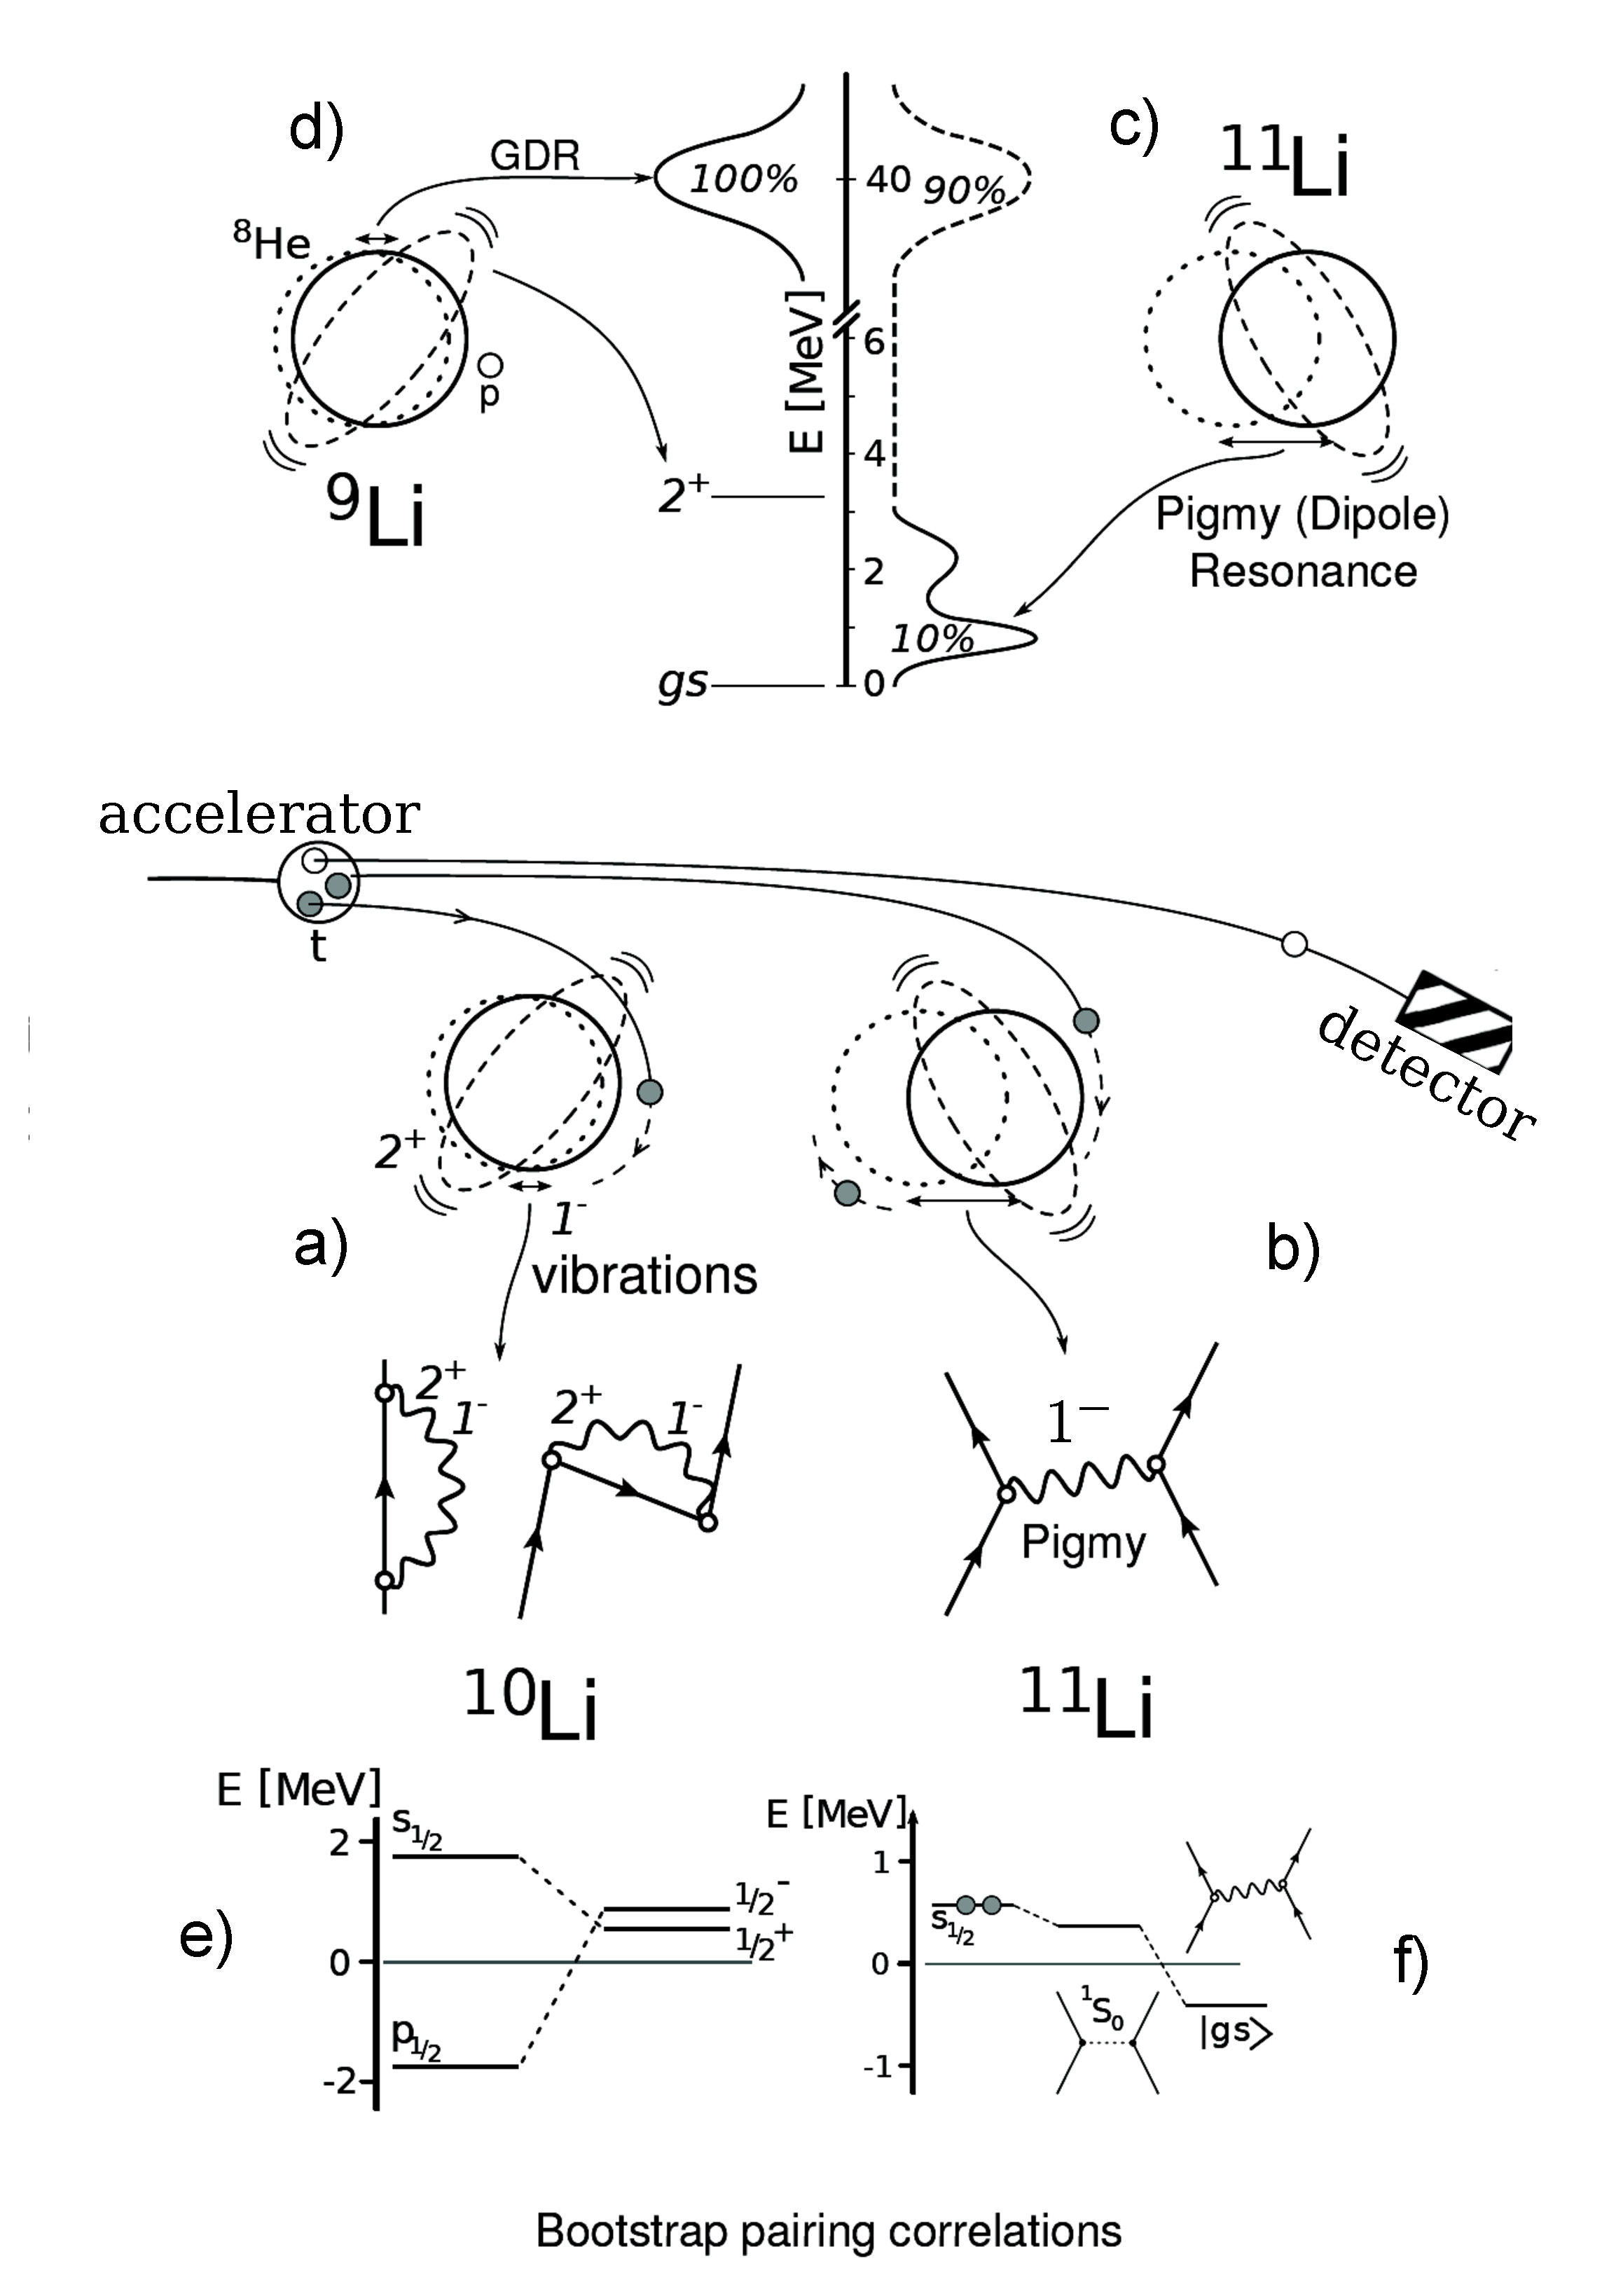
\includegraphics[width=0.75\textwidth]{C8/figsC8/BootStrap_Li}
	\end{center}
	\caption{Schematic representation of the collective quadrupole and dipole response of litium isotopes, and of a ($t,p$) reaction (in the text one reasons in terms of flux of low energy neutrons) in which two neutrons are transfered to $^9$Li (see also Fig. \ref{fig8_1_2}).}
\label{fig8_A_1}
\end{figure}
Such possibility implies that, for a short time, of the order of the traversal time, the two (unbound) neutrons will move in a gas of virtual bosonic excitations, also made out of dipole pigmy resonances. Consequently, they can get dressed becoming heavier (lighter), as well as getting correlated by exchanging  these bosonic collective vibrations. 
The first phenomenon is associated, as discussed above, with phononic backflow (Pauli principle upflow) leading to $^{10}$Li-like quasi-bound ($s-$wave) and resonant ($p-$wave) dressed single-particle states displaying parity inversion.
The second phenomenon, mediated by phonon exchange between halo neutrons, contributes in a major way to the glue which binds the neutron halo Cooper pair to the $^{9}$Li core. Within the above scenario, one can posit that the $^{11}$Li dipole pigmy resonance can hardly be viewed but in symbiosis with the $^9$Li halo neutron pair addition mode. The above described bootstrap phonon-exchange mechanism can be viewed as a novel microscopic embodiment of the Bardeen--Pines--Fr\"{o}lich-like processes to spontaneously break gauge invariance\footnote{Bootstrapping or booting. The term is often attributed to Rudolf Erich Raspe's story The surprising Adventures of Baron M\=unchausen, where the main character pulls himself out of a swamp by his hair. Early 19th century USA: ``pull oneself over a fence by one's bootstraps''}.


To conclude, let us comment on Fig. \ref{fig8_A_1}. As said above, (a) the dressing of single--particle levels by collective vibrations and (b) the renormalization of the bare $NN$--interaction, in particular of the pairing interaction, through the exchange of these modes between nucleons moving in time reversal states lying close to the Fermi energy, play a central role in nuclear structure. In particular, in the case of the single Cooper pair system $^{11}$Li, most of the glue is provided by the exchange of the pigmy resonance, namely a low--lying isovector dipole vibration. The pigmy resonance (c) is a chunk of the GDR of the core $^9$Li (d) and arises from radial inhomogeneous damping. This mode is intimately related to the spontaneous symmetry breaking of space homogeneity associated with the fact that the center of mass of a finite system like the atomic nucleus, specifies a privileged position in space. While $^9_3$Li$_6$ is bound, $^{10}_3$Li$_7$ is not. (e) through renormalization processes, the $p_{1/2}$ bound state is shifted to higher energies from that predicted by a standard mean field potential, while the $s_{1/2}$ continuum state is lowered to an energy close,  below that of the $p_{1/2}$ state. (f) While the screened bare pairing interaction is subcritical, the exchange of vibrations between the halo neutrons is able to, weakly, bind the system.






\section{Table 1 PRL}\label{C8AppB}
The $1/2^-$ (2.69 MeV) first excited state of $^9$Li can in principle, not only be populated through a two--particle transfer process, but also through a break up process in which one (see Fig. \ref{fig8_B_1}(f)), or both neutrons (see Fig. \ref{fig8_B_1}(g)) are forced into the continuum for then eventually one of them to fall into the $1p_{3/2}$ orbital of $^9$Li and excite the quadrupole vibration of the core (\cite{Potel:10}), in keeping with the fact that the main RPA amplitude of this state is precisely $X(1p^{-1}_{3/2},1p_{1/2})(\approx 1)$ (cf. ref \cite{Barranco:01}). The remaining channel populating the first excited state of $^9$Li is associated with an inelastic process (see Fig. \ref{fig8_B_1}(h)): two--particle transfer to the ground state of $^{9}$Li and Final State (inelastic scattering) Interaction (FSI) between the outgoing triton and $^{9}$Li in its ground state, resulting in the inelastic excitation of  the $1/2^-$ state.


Making use of the wavefunctions of  \cite{Barranco:01} and of a software developed on purpose to take into account microscopically all the different processes mentioned above, that is 9 different reaction channels (cf. caption to Table \ref{tab8_B_1}) and continuum states up to 50 MeV of excitation energy, the corresponding transfer amplitudes and associated probabilities $p_l$ were calculated.


 In Table \ref{tab8_B_1} are displayed the probabilities $p_l=|S_l^{(c)}|^2$ associated with each of the processes discussed above, where the amplitude $S_l^{(c)}$ is related to the total cross section associated with each of the channels $c$  by the expression \citep{Satchler:80,Landau:81}
\begin{equation}\label{eq6}
    \sigma_c=\frac{\pi}{k^2}\sum_l(2l+1)|S_l^{(c)}|^2,
\end{equation}
$k$ being the wave number of the relative motion between the reacting nuclei.



%%
 In keeping with the small values of $p_l$, in what follows we take into account the interference between the contributions associated with the different reaction paths making use of second order perturbation theory, instead of a coupled channel treatment (cf. e.g.  \cite{Ascuitto:69} \cite{Tamura:70} \cite{Khoa:04} \cite{Keeley:07b} \cite{Thompson:88}). In particular in the case of the $1/2^-$ (2.69 MeV) first excited state of $^9$Li,
\begin{equation}
    \frac{d\sigma}{d\Omega}(\theta)=\frac{\mu^2}{16\pi^3\hbar^4}\left|\sum_l(2l+1)P_l(\theta)\sum_{c=2}^5 T^{(c)}_l\right|^2,
\end{equation}
where $\mu$ is the reduced mass and $T^{(c)}_l$ are the transition matrix elements (in the DWBA \cite{Satchler:80}) associated with the different channels and for each partial wave.

\begin{table}
\begin{center}
\begin{tabular}{|c|c|c|c|c|c|}
\hline
\backslashbox {$l$}{$c$} & \textbf{1} & \textbf{2} & \textbf{3} & \textbf{4}& \textbf{5} \\
\hline
 0& $4.35\times 10^{-3}$ &$1.79\times 10^{-4}$ & $4.81\times 10^{-6}$& $2.90\times 10^{-11}$& $3.79\times 10^{-8}$\\
\hline
 1& $3.50\times 10^{-3}$& $9.31\times 10^{-4}$& $1.47\times 10^{-5}$&$1.87\times 10^{-9}$& $1.09\times 10^{-6}$\\
\hline
 2& $7.50 \times 10^{-4}$& $8.00\times 10^{-5}$& $2.45\times 10^{-5}$&$1.25\times 10^{-8}$&$1.21\times 10^{-6}$\\
\hline
 3& $6.12\times 10^{-4}$&$9.81\times 10^{-5}$ & $1.51\times 10^{-6}$&$6.50\times 10^{-10}$&$2.20\times 10^{-7}$\\
\hline
 4&$1.10\times 10^{-4}$ &$ 1.18\times 10^{-5}$ & $2.21\times 10^{-7}$&$4.80\times 10^{-11}$&$1.46\times 10^{-8}$ \\
\hline
 5& $3.65\times 10^{-5}$& $2.16\times 10^{-7}$& $7.42\times 10^{-9}$&$6.69\times 10^{-13}$&$9.63\times 10^{-10}$\\
\hline
 6& $1.35\times 10^{-5}$& $6.05\times 10^{-8}$&$2.88\times 10^{-10}$ &$8.04\times 10^{-15}$&$1.08\times 10^{-11}$\\
\hline
 7& $4.93\times 10^{-6}$& $7.78\times 10^{-8}$& $6.01\times 10^{-11}$&$4.05\times 10^{-16}$&$5.26\times 10^{-13}$\\
\hline
 8& $2.43\times 10^{-6}$& $2.62\times 10^{-8}$& $7.4\times 10^{-12}$&$1.26\times 10^{-17}$&$9.70\times 10^{-11}$\\
\hline
\end{tabular}
\caption{Probabilities $p_l$  associated with the processes described in the text for each partial wave $l$. The different channels are labeled by a channel number $c$ equal to: \textbf{1}, multistep transfer to the $^9$Li ground state (Fig. \ref{fig8_B_1}(d)); \textbf{2}, multistep transfer (Fig. \ref{fig8_B_1}(e)) to the first excited $^9$Li state, \textbf{3}, breakup (Fig. \ref{fig8_B_1}(f)), \textbf{4}, breakup  (Fig. \ref{fig8_B_1}(g)), and \textbf{5} inelastic processes (Fig. \ref{fig8_B_1}(h)) involved in the population of the $1/2^-$ (2.69 MeV) first excited state of $^9$Li. Of notice that the probabilities displayed in columns \textbf{1} and \textbf{2} result from the (coherent) sum of three amplitudes namely those associated with successive, simultaneous and non--orthogonality transfer channels (see also Fig. \ref{fig8_B_3}) after \cite{Potel:10}.}\label{tab8_B_1}
\end{center}
\end{table}


 Making use of all the elements discussed above, multistep transfer (see e.g. \cite{Bayman:82}, \cite{Igarashi:91},  \cite{Bayman:73} as well as \cite{Broglia:04a}), breakup and inelastic channels were calculated, and the results displayed in Figs. \ref{fig8_B_2} and \ref{fig8_B_3} and in Table \ref{tab8_B_1}. Theory provides an overall account of the experimental findings. In particular, in connection with the $1/2^-$ state, this result essentially emerges from cancellations and coherence effects taking place between the three terms contributing to the multistep two--particle transfer cross section (see Fig. \ref{fig8_B_3}), tuned by the nuclear structure amplitudes associated with the process shown in Fig. \ref{fig8_B_1} (e) as well as Eqs. (\ref{eq8_2_1})--(\ref{eq8_2_3}). In fact, and
as shown in Figs. \ref{fig8_B_2} and \ref{fig8_B_3}, the contributions of break up processes and inelastic   (Figs. \ref{fig8_B_1}(f),(g) and (h) respectively) to the population of the $1/2^-$ (2.69 MeV) first excited state of $^9$Li are negligible as compared with the process depicted in Fig. \ref{fig8_B_1}(e). In the case of the breakup channel (Figs. \ref{fig8_B_1}(f) and \ref{fig8_B_1}(g)) this is a consequence of the low bombarding energy of the $^{11}$Li beam (inverse kinematics), combined with the small overlap between continuum (resonant) neutron $p_{1/2}$ wavefunctions and  bound state wavefunctions. In the case of the inelastic process (Fig. \ref{fig8_B_1}(h)), it is again a consequence of the relative low bombarding energy. In fact, the adiabaticity parameters $\xi_C,\xi_N$ (see eqs. (IV.12) and (IV.14) of ref. \cite{Broglia:04a}) associated with Coulomb excitation and inelastic excitation in the t+$^9$Li channel are larger than 1, implying an adiabatic cutoff. In other words, the quadrupole mode is essentially only polarized during the reaction but not excited. The situation is quite different in the case of the intervening of the virtual processes  displayed in Fig. \ref{fig8_B_1} (b) and (c) leading to the population of the $1/2^-$ state displayed in Fig. \ref{fig8_B_1} (e). Being those off--the--energy shell processes, energy is not conserved, and adiabaticity gets profoundly modified.

  \begin{figure}
  \centerline{\includegraphics*[width=12cm,angle=0]{C8/figsC8/fig8_B_1x}}
  	\caption{Representative Nuclear Field Theory--Feynman diagrams associated with correlation process ((a),(b),(c)) and with one-- and two--particle pick--up reactions ((i),(j) and (d),(e) respectively) of the halo neutrons of $^{11}$Li (Cooper pair, indicated in terms of a double arrowed line). Also shown are the possible diagrams associated with other channels (breakup and inelastic) populating the $1/2^-$ (2.69 MeV) state: f) one of the halo neutrons is picked up (the other one going into the continuum, i.e. breaking up from the $^9$Li core) together with a neutron from the $p_{3/2}$ orbital of the $^9$Li core  leading eventually to the excitation of the $1/2^-$ final state ($2^+$ density mode (wavy line) coupled to the $p_{3/2}(\pi)$), g) the proton field acting once breaks the Cooper pair forcing one of the halo neutrons to populate a $p_{1/2}$ continuum state (the other one follows suit), while acting for the second time picks up one of the neutrons moving in the continuum and another one from those moving in the $p_{3/2}$ orbital of $^9$Li eventually leaving the core in the quadrupole mode of excitation. In (h) the  two--step transfer to the $^9$Li ground state plus the inelastic final channel process exciting the $(2^+\otimes p_{3/2}(\pi))_{1/2^-}$ state is shown. After \cite{Potel:10}.}\label{fig8_B_1}
  \end{figure}
    \begin{figure}
    \centerline{\includegraphics*[width=12cm,angle=0]{C8/figsC8/fig8_B_2}}
    	\caption{Experimental (\cite{Tanihata:08}) and theoretical differential cross sections (including multistep transfer as well as breakup and inelastic channels, \cite{Potel:10}).  of the
    	$^1$H($^{11}$Li,$^9$Li)$^3$H  reaction populating the ground state ($3/2^-$) and the first excited state ($1/2^-$; 2.69 MeV) of $^{9}$Li. Also shown (dash--dotted curve) is the differential cross section associated with this state but taking into account only multistep transfer. The optical potentials used are from \citep{Tanihata:08,An:06}. The absolute cross sections associated with the ground state ($3/2^-$) is predicted to be 6.1 mb ($6.7\pm 0.9$ mb) while that corresponding to the first excited state ($1/2^-; 2.69$ MeV) being 0.7 mb ($1.0\pm 0.36$ mb). }\label{fig8_B_2}
    \end{figure}
        \begin{figure}
        \centerline{\includegraphics*[width=12cm,angle=0]{C8/figsC8/fig8_B_3}}
        	\caption{Successive, simultaneous and non-orthogonality contributions (prior representation)
        	to the  $^1$H($^{11}$Li,$^9$Li)$^3$H differential cross section
        	associated with the population of the $1/2^-$ state
        	of $^9$Li, displayed in Fig. \ref{fig8_B_2}. Also shown is the (coherent) sum of the breakup ($c=3$ and 4) and inelastic ($c=5$) channel contributions.}\label{fig8_B_3}
        \end{figure}
\section[Formfactors for the reaction $^1$H($^{11}$Li,$^9$Li)$^3$H]{Modified formfactor associated with the reactions $^1$H($^{11}$Li,$^9$Li(gs))$^3$H and $^1$H($^{11}$Li,$^9$Li(1/2$^-$; 2.69 MeV)$^3$H state}\label{C8AppC}
\section{Software}\label{C8AppD}
In this Appendix we provide a brief description of the numerical methods implemented in the code written to evaluate the differential cross sections. The two--nucleon transfer differential cross section is given by Eq. (\ref{eq5.1.4}),  so the principal task consist in calculating the transfer amplitudes $T^{(1)}(\theta),T^{(2)}_{succ}(\theta)$ and $T^{(2)}_{NO}(\theta)$ described in Eqs. \ref{eq1_40}--\ref{eq1_42}, by numerically evaluating the corresponding integrals.  The dimensionality of the integrals  can be reduced by expanding in partial waves (eigenfunctions of the angular momentum operator) the distorted waves and wavefunctions present in the corresponding integrands. The resulting expressions are Eqs. (\ref{eq111}) and (\ref{eq112}) for $T^{(1)}(\theta)$, Eqs. (\ref{eq27}), (\ref{eq121}) and (\ref{eq122}) for $T^{(2)}_{succ}(\theta)$, and Eqs. (\ref{eq138}), (\ref{eq139}) and (\ref{eq140}) for $T^{(2)}_{NO}(\theta)$. The integrals are computed numerically with the method of Gaussian quadratures. 


The one--dimensional (radial) functions appearing in the integrands are defined in a spatial grid up to a given maximum radius $r_{max}$. The bound state  wavefunctions are obtained by numerical integration of the radial Schr\"odinger equation for a Woods--Saxon potential with a spin--orbit term. The parameters defining the shape of the potential are given as an input, while the depth is adjusted to reproduce the binding energy of the state under consideration. The resulting potential corresponding to the final (initial) nucleon bound state stands also for the interaction potential featured in the integrand in the prior (post) representation. The distorted waves are obtained by integrating the radial Schr\"odinger equation with positive energy from $r=0$ to $r_{max}$, and matching the solution with the corresponding Coulomb wave function at a given $r=r_{match}$, big enough to lie outside of the range of the nuclear interaction. The  Woods--Saxon optical potentials  used to obtain the distorted waves consist on a real Coulomb term, a real and imaginary volume terms, an imaginary surface term, and a real and imaginary spin orbit terms. The parameters needed to specify all those terms are given as an input.  




   
\section{Articulo Belyaev Pairing vibrational band based on $N=6$.}\label{C8AppE}
\section{Simple estimates revisited.}\label{App6F}
\section{Statistics.}\label{App6G}
Let us consider two identical particles moving in a one--dimensional harmonic oscillator. Let us assume  that one is in the ground state and the other  is in the first excited state. According to the superposition principle 
\begin{align}\label{eqApp6G1}
\Phi(x_1,x_2)=\lambda\phi_1(x_1)\phi_0(x_2)+\mu\phi_0(x_1)\phi_1(x_2).
\end{align} 
Let us calculate the correlation of these particles, that is, the quantity
\begin{align}\label{eqApp6G2}
C=\frac{\langle x_1x_2\rangle-\langle x_1\rangle\langle x_2\rangle}{\sqrt{\left(\langle x_1^2\rangle-\langle x_1\rangle^2\right)\left(\langle x_2^2\rangle-\langle x_2\rangle^2\right)}}
\end{align} 
Let us start with
\begin{align}\label{eqApp63}
\nonumber\langle x_1x_2\rangle=&\int dx_1 dx_2 \left(\lambda^*\phi_1^*(x_1)\phi_0^*(x_2)+\mu^*\phi_0^*(x_1)\phi_1^*(x_2)\right)\\
\nonumber&\times(x_1 x_2)\left(\lambda\phi_1(x_1)\phi_0(x_2)+\mu\phi_0(x_1)\phi_1(x_2)\right)\\
\nonumber &=|\lambda|^2\langle\phi_1|x_1|\phi_1\rangle\langle\phi_0|x_2|\phi_0\rangle+\lambda^*\mu\langle\phi_1|x_1|\phi_0\rangle\langle\phi_0|x_2|\phi_1\rangle\\
&+\lambda\mu^*\langle\phi_0|x_1|\phi_1\rangle\langle\phi_1|x_2|\phi_0\rangle+|\mu|^2\langle\phi_0|x_1|\phi_0\rangle\langle\phi_1|x_1|\phi_1\rangle\langle\phi_0|x_1|\phi_0\rangle\langle\phi_1|x_1|\phi_1\rangle
\end{align} 

In keeping with the fact that

\begin{align}\label{eqApp6G4}
\langle\phi_1|x|\phi_1\rangle=\langle\phi_0|x|\phi_0\rangle=0,
\end{align} 
and
\begin{align}\label{eqApp6G5}
\langle\phi_0|x|\phi_1\rangle=\langle\phi_1|x|\phi_0\rangle=\sqrt{\frac{\hbar\omega}{2C}},
\end{align}
one obtains
\begin{align}\label{eqApp6G6}
\langle x_1x_2\rangle=\left(\frac{\hbar\omega}{2C}\right)\Re(\lambda^*\mu).
\end{align} 
And 
\begin{align}\label{eqApp6G7}
\sqrt{\quad}=\left(\frac{\hbar\omega}{2C}\right),
\end{align}
for the denominator of Eq. (\ref{eqApp6G2}).
From the above results the correlation function between particle 1 and 2 is
\begin{align}\label{eqApp6G8}
C=\frac{2C}{\hbar\omega}\langle x_1x_2\rangle=2\Re(\lambda^*\mu)=
\left\{
\begin{array}{c}
 1\quad (\lambda=+\mu=\frac{1}{\sqrt{2}})\\ 
 -1 \quad (\lambda=-\mu=\frac{1}{\sqrt{2}})
\end{array}
\right. 
\end{align}
It is of notice that, in quantum mechanics, average values imply the mean outcome of a large number of experiments. In this case, of the (simultaneous) measure of the position of the two particles (cf. \cite{Basdevant:05}).






\section{Correlation length and quantality parameter.}\label{App6H}
The correlation length can be defined as
\begin{align}\label{eqApp6H1}
\xi=\frac{\hbar v_F}{2\Delta}\approx\frac{\hbar^2}{m}\frac{k_F}{2\Delta}
\end{align}
where the Fermi momentum in the case of stable nuclei lying along the stability valley is
\begin{align}\label{eqApp6H2}
k_F\approx 1.36\,\text{fm}^{-1}.
\end{align}
Thus,
\begin{align}\label{eqApp6H3}
\xi=20\,\text{MeV fm}^2\times \frac{1.36}{\Delta}\,\text{fm}^{-1}\approx \frac{27}{\Delta}\,\text{fm},
\end{align}
and,
\begin{align}\label{eqApp6H4}
\xi\approx 27\,\text{fm},\quad (\Delta\approx1\,\text{MeV}).
\end{align}
Let us now define,
\begin{align}\label{eqApp6H5}
k_F\approx\frac{a}{\xi}=1.36\,\text{fm}^{-1}
\end{align}
obtaining, 
\begin{align}\label{eqApp6H6}
a\approx 37;\quad k_F\approx \frac{37}{\xi}.
\end{align}  
One can then write,
\begin{align}\label{eqApp6H7}
1=\left(\frac{\hbar^2}{m\xi^2}\right)\left(\frac{1}{2\Delta}\right)37=q\times 37,
\end{align} 
where the quantality parameter is, in the present case,
\begin{align}\label{eqApp6H8}
q\approx0.03.
\end{align} 
That is, the two partner nucleons are, in the Cooper pair, rigidly anchored.

We now consider $^{11}$Li, and calculate $k_F$ (neutrons) with the help of the Thomas--Fermi model, 
\begin{align}\label{eqApp6H9}
k_F=\left(3\pi^2\frac{8}{\frac{4\pi}{3}(4.58)^3}\right)^{1/3}\,\text{fm}^{-1}\approx\frac{(18\pi)^{1/3}}{4.58}\,\text{fm}^{-1}\approx 0.84\,\text{fm}^{-1}.
\end{align} 
The correlation length is,
\begin{align}\label{eqApp6H10}
\xi\approx\frac{\hbar^2}{m}\frac{k_F}{2E_{corr}}\approx 20\,\text{MeV fm}^{-1}\approx 42\,\text{fm},
\end{align} 
and
\begin{align}\label{eqApp6H11}
k_F=\frac{a}{\xi}\approx \frac{a}{42\,\text{fm}}=0.84\,\text{fm}^{-1};\quad a\approx 35; \quad k_F=\frac{35}{\xi},
\end{align} 
leading to
\begin{align}\label{eqApp6H12}
1=\left(\frac{\hbar^2}{m\xi^2}\right)\left(\frac{1}{2E_{corr}}\right)35=q\times 35,
\end{align}
and of the resulting quantality parameter,
\begin{align}\label{eqApp6H13}
q\approx 0.03.
\end{align}
It is of notice that this result is but an alternative embodiment of the relation (\ref{eq3.3.8}). Now, one could argue that both (\ref{eq3.3.8}) and (\ref{eqApp6H13}) (as well as (\ref{eqApp6H8}) for stable nuclei), are just a manifestation of (\ref{eqApp6G8}). That there is more to it is forcefully expressed by the fact that, selecting $|s_{1/2}^2(0)\rangle$ ($|p_{1/2}^2(0)\rangle$) as the Cooper pair of $^{11}$Li leads to absolute two--particle transfer cross sections which are about one order of magnitude larger (smaller) than the observed cross section (see Fig. \ref{fig8_1_2}). The fact that the NFT result (\ref{eq8_2_1})--(\ref{eq8_2_3}) with its unusual pigmy binding and parity inversion clothing mechanism reproduces observations within experimental errors, underscores the central role played by structure on Cooper pair tunneling, through the emergent property of generalized pairing rigidity.


Summing up pairing, both bare $NN$-- and long range induced interaction changes the statistics of the elementary modes from fermionic to bosonic and, at the same time, the value of the quantality parameter from $q\approx1$ to $q\ll 1$ (delocalized $\rightarrow$ rigidly anchored to the Cooper pair) thus leading to a generalized gauge rigidity, the detailed renormalizing and dressing mechanisms ultimately deciding on the soundness and applicability of the description under discussion. The fact that in working out the reaction mechanism one uses, for practical reasons, a single--particle basis (second order DWBA corrected by non--orthogonality), reconstructing the interweaving of these particles with the collective modes in term of sums over virtual states, does not alter the physics embodied in the NFT solutions. Rather, it provides its confirmation (Fig. \ref{fig8_1_2}).
 
\section{$k$--mass in $^{11}$Li and Pauli principle.}\label{App6I}














\end{subappendices}
\bibliographystyle{abbrvnat}
%\bibliography{C:/Gregory/Broglia/notas_ricardo/nuclear_bib}
 \bibliography{../nuclear_bib}